\usetikzlibrary{calc}


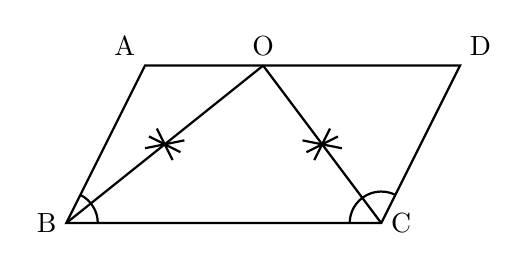
\begin{tikzpicture}[scale=1]

    % Define the vertices of the parallelogram
    \coordinate (B) at (0,0);
    \coordinate (C) at (4,0);
    \coordinate (D) at (5,2);
    \coordinate (A) at (1,2);

    % Draw the parallelogram
    \draw[thick] (A) -- (B) -- (C) -- (D) -- cycle;

    % Define the intersection point O of the angle bisectors
    % This is approximately in the middle of the top edge
    \coordinate (O) at (2.5,2);

    % Draw the angle bisectors from B and C to O
    \draw[thick] (B) -- (O);
    \draw[thick] (C) -- (O);

    % Draw the single angle arc at B (from line BC to line BA)
    \draw[thick] (B) ++(0:0.4) arc (0:63.4:0.4);

    % Draw the single angle arc at C (extended to line CD)
    % It starts from CB (180 degrees) and ends at CD (63.4 degrees)
    \draw[thick] (C) ++(180:0.4) arc (180:63.4:0.4);

    % Add the tick marks on the bisector lines
    % Tick marks on BO
    \coordinate (M1) at ($ (B)!0.5!(O) $);
    \draw[thick] ($ (M1) + (-0.1,0.2) $) -- ($ (M1) + (0.1,-0.2) $);
    \draw[thick] ($ (M1) + (-0.2,0.1) $) -- ($ (M1) + (0.2,-0.1) $);
    \draw[thick] ($ (M1) + (-0.25,-0.05) $) -- ($ (M1) + (0.25,0.05) $);

    % Tick marks on CO
    \coordinate (M2) at ($ (C)!0.5!(O) $);
    \draw[thick] ($ (M2) + (-0.1,-0.2) $) -- ($ (M2) + (0.1,0.2) $);
    \draw[thick] ($ (M2) + (-0.2,-0.1) $) -- ($ (M2) + (0.2,0.1) $);
    \draw[thick] ($ (M2) + (-0.25,0.05) $) -- ($ (M2) + (0.25,-0.05) $);

    % Add labels for the vertices
    \node[above left] at (A) {A};
    \node[left] at (B) {B};
    \node[right] at (C) {C};
    \node[above right] at (D) {D};
    \node[above] at (O) {O};

\end{tikzpicture}